
\section{\label{sec:A-Formal-Description}A Formal Description of Backbone}

In this section we formally describe how components, defined in an
extension stratum using a combination of resemblance and replacement,
can evolve the existing compositional structure of an architecture
defined in a base stratum.

The ability to evolve an architecture in a decentralized manner, where
strata are used to group and organise these component definitions,
leads naturally to the desire to combine and merge strata that each
evolve a common base into a unified architecture. We describe the
merging rules, showing that any structural errors can be corrected
by adding further component definitions.

To make the treatment more concrete we present a variant of our bridge
system (figure \ref{fig:A-variant-of}) and demonstrate how the formal
model applies to this architecture. We have (\texttt{MULTISLB} resembles
\texttt{SLB}), (\texttt{SLBa\textquoteright{}} evolves \texttt{SLB})
and (\texttt{SLBb\textquoteright{}} evolves \texttt{SLB}). In other
words, the three middle strata represent branches of the original
system. The top stratum has visibility of all branches and hence merges
these, bringing the definitions into one place with potential conflicts.

\begin{figure}[h]
\noindent \begin{centering}
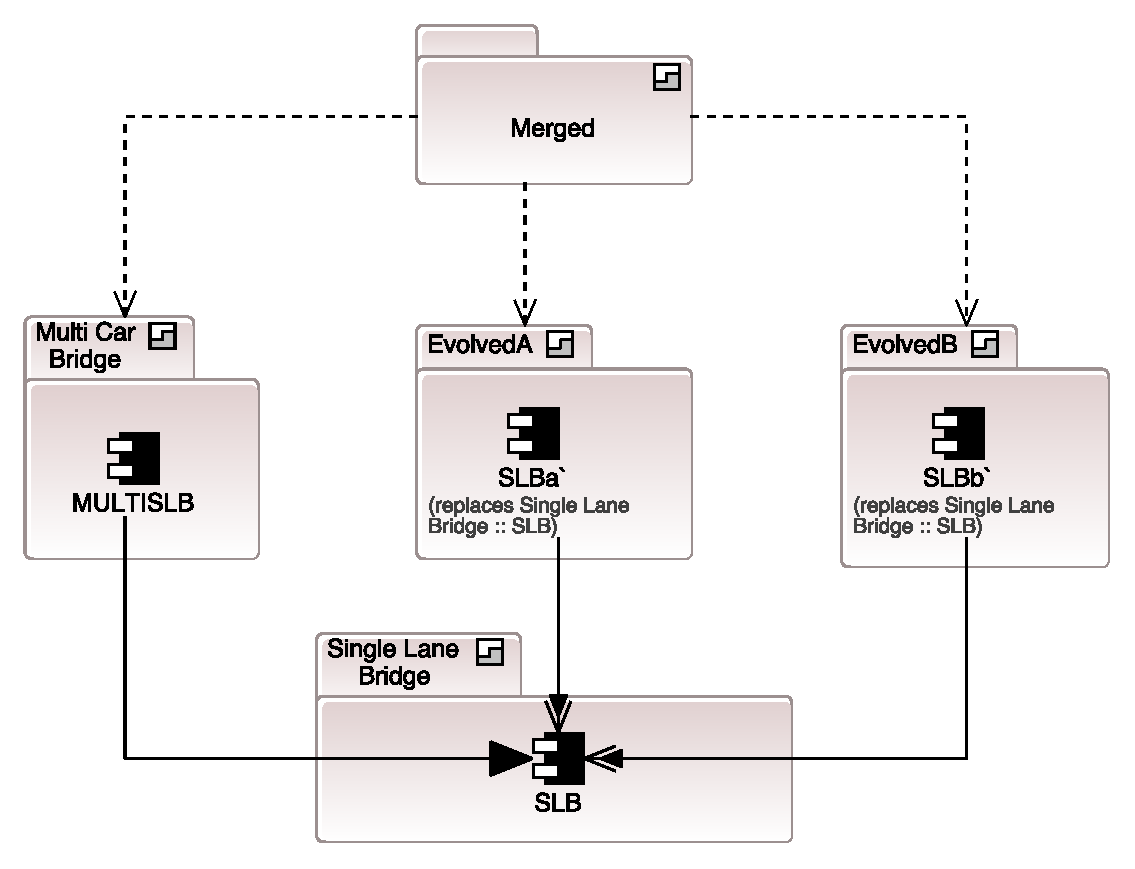
\includegraphics[width=0.8\columnwidth]{images/formal-merged}
\par\end{centering}

\protect\caption{\label{fig:A-variant-of}A variant of the Bridge system}


\end{figure}


The formal model is specified in Alloy \cite{Jackson2006,Jackson2002},
which is a relational logic supported by model checking tools. The
full specification is presented in the appendix at the end of this
report. Dependencies between strata in an extension architecture govern
the order of application of resemblance and replacement. We therefore
begin by describing the stratum concept.


\subsection{Structures}
\begin{lyxlist}{00.00.0000}
\item [{\emph{Definition}}] A \emph{stratum} is a hierarchical module that
owns and groups elements (component and interface) definitions.
\end{lyxlist}
A stratum may depend on a set of other strata and it owns a set of
elements. An element is an abstraction of a component or interface
or other compositional artifact. We model stratum as below.
\begin{lyxcode}
{\footnotesize{}sig~Stratum~\{}{\footnotesize \par}

{\footnotesize{}~~dependson:~set~Stratum,}{\footnotesize \par}

{\footnotesize{}~~elements:~set~Element,}{\footnotesize \par}

{\footnotesize{}~~...~\}}{\footnotesize \par}
\end{lyxcode}
Transitive strata dependencies determine which other elements are
visible to elements in that stratum for use in composition, resemblance
and replacement relationships.

We outlaw circular dependencies between strata, forcing the structure
into a graph.
\begin{lyxcode}
{\footnotesize{}all~s:~Stratum~|~s~not~in~s.\textasciicircum{}dependson}{\footnotesize \par}
\end{lyxcode}
This allows us to divide strata into those a given stratum depends
on (transitively), those that depend on it, and those it has no visibility
of.

Two strata are termed independent if they have no visibility of each
other. If independent strata depend on common underlying strata, like
\texttt{EvolvedA} and \texttt{EvolvedB} in figure X, we call them
branches.
\begin{lyxcode}
{\footnotesize{}pred~branch{[}a,~b:~Stratum{]}~\{}{\footnotesize \par}

{\footnotesize{}~~let~alla~=~a.{*}dependson,~allb~=~b.{*}dependson~|}{\footnotesize \par}

{\footnotesize{}~~~~a~not~in~allb~and~b~not~in~alla~and}{\footnotesize \par}

{\footnotesize{}~~~~~~some~alla~\&~allb}{\footnotesize \par}

{\footnotesize{}\}}{\footnotesize \par}\end{lyxcode}
\begin{lyxlist}{00.00.0000}
\item [{\emph{Definition}}] An \emph{element} is a compositional structure,
such as a component or interface, that can participate in resemblance
and replacement relationships.
\end{lyxlist}
It is represented by the following structure.
\begin{lyxcode}
{\footnotesize{}sig~Element~\{}{\footnotesize \par}

{\footnotesize{}~~home:~Stratum,}{\footnotesize \par}

{\footnotesize{}~~resembles:~set~Element,}{\footnotesize \par}

{\footnotesize{}~~replaces:~lone~Element,}{\footnotesize \par}

{\footnotesize{}~~deltas:~lone~Deltas}{\footnotesize \par}

{\footnotesize{}\}}{\footnotesize \par}
\end{lyxcode}
Each element has a single home stratum, which owns it, in accord with
the \texttt{Stratum::elements} set. An element can resemble any number
of other elements of the same type that are visible to, or in, the
home stratum, and optionally replace an element from a stratum that
the home (transitively) depends upon.

As seen below, we disallow having both the initial definition of an
element and its replacement in the same home. This is because stratum
is a unit of solitary development ownership - if the owner (person
or group) of a stratum wished to adjust the structure of an owned
component, they would edit the definition directly rather than creating
a replacement. Element replacement conversely allows developers to
make adjustments to strata they do not have ownership of.
\begin{lyxcode}
{\footnotesize{}all~e:~Element~|}{\footnotesize \par}

{\footnotesize{}~~~~let~res~=~e.resembles,~rep~=~e.replaces~|}{\footnotesize \par}

{\footnotesize{}~~res.home~in~e.home.{*}dependson}{\footnotesize \par}

{\footnotesize{}~~~~and~rep.home~in~e.home.\textasciicircum{}dependson}{\footnotesize \par}

{\footnotesize{}~~~~and~e~not~in~res~}{\footnotesize \par}\end{lyxcode}
\begin{lyxlist}{00.00.0000}
\item [{\emph{Definition}}] A \emph{deltas} structure holds the adds, deletes
or replacements to the resembled constituent structure of an element\footnote{There are two types of replacement in Backbone: element replacement
where one element can be substituted for another, and delta replacement
where an element definition replaces some of the constituents that
have been inherited via resemblance. Here we are talking about the
latter concept.}
\end{lyxlist}
We model deltas as shown. Note that a constituent is a building block
of an element. In the case of a component, this could be a port, a
connector, an attribute or a part. Other than having an identity,
constituent in our specification is just a placeholder.
\begin{lyxcode}
{\footnotesize{}sig~Deltas~\{}{\footnotesize \par}

{\footnotesize{}~~owner:~Element,}{\footnotesize \par}

{\footnotesize{}~~add,~delete:~set~Constituent,}{\footnotesize \par}

{\footnotesize{}~~replace:~Constituent~->~Constituent}{\footnotesize \par}

{\footnotesize{}\}}{\footnotesize \par}
\end{lyxcode}
The \texttt{add} and \texttt{delete} fields indicate constituents
to add or delete. The \texttt{replace} field is a relation fom the
constituent being replaced to that replacing it. A key point is that
any replacing constituent assumes the identity of the replaced one
- this allows connectors and other references to the replaced item
to stay valid.

If an element does not resemble another then all the deltas will be
adds which build up the initial structure.


\subsection{The Expanded Resemblance Graph}
\begin{lyxlist}{00.00.0000}
\item [{\emph{Definition}}] The \emph{expanded resemblance graph} is a
resemblance graph for a given element from a given stratum perspective,
which takes into account any replacements visible from that perspective.
\end{lyxlist}
The expanded resemblance graph is the resemblance graph for an element
after all the replacements from extension strata have been factored
in.

Consider, for example, that the \texttt{MULTISLB} non-expanded resemblance
graph is (\texttt{MULTISLB} resembles \texttt{SLB}). If we compute
the expanded resemblance graph from the perspective of \texttt{Merged},
then we need to take into account that two additional replacements
(evolutions) are present. From this perspective, the expanded resemblance
graph would now look like (\texttt{MULTISLB} resembles \texttt{SLBa\textquoteright{}}
+ \texttt{SLBb\textquoteright }, \texttt{SLBa\textquoteright{}} resembles
\texttt{SLB}, \texttt{SLBb\textquoteright{}} resembles \texttt{SLB}).
This is shown graphically in figure \ref{fig:The-expanded-resemblance}.

\begin{figure}[h]
\noindent \begin{centering}
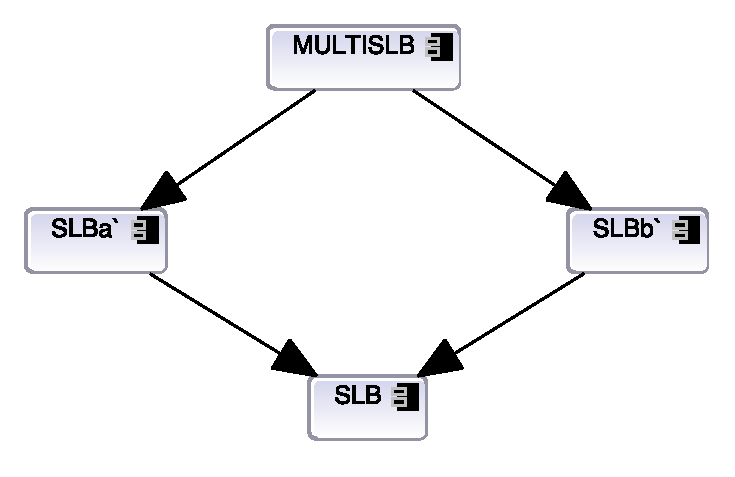
\includegraphics[width=0.6\columnwidth]{images/formal-expanded}
\par\end{centering}

\protect\caption{\label{fig:The-expanded-resemblance}The expanded resemblance graph
for \texttt{MULTISLB}}


\end{figure}


From the same perspective, consider that \texttt{SLB} has a two headed
expanded resemblance graph, reflecting that \texttt{SLBa\textquoteright{}}
and \texttt{SLBb\textquoteright{}} have no direct visibility of each
other. If these definitions conflict then any issues could be corrected
by a new evolution in the \texttt{Merged} stratum which could add,
delete or replace constituents to ensure well formedness. Similarly,
it may be the case from the \texttt{Merged} perspective that evolutions
to \texttt{SLB} invalidate the \texttt{MULTISLB} definition. Again,
any issues can be rectified using evolutions in \texttt{Merged}. For
instance, if we have both an evolution of \texttt{SLB} to correct
the merged definition, and a further evolution to \texttt{MULTISLB}
then the expanded graph for \texttt{MULTISLB} would look as shown
in figure \ref{fig:Correcting-any-compositional}.

\begin{figure}[h]
\noindent \begin{centering}
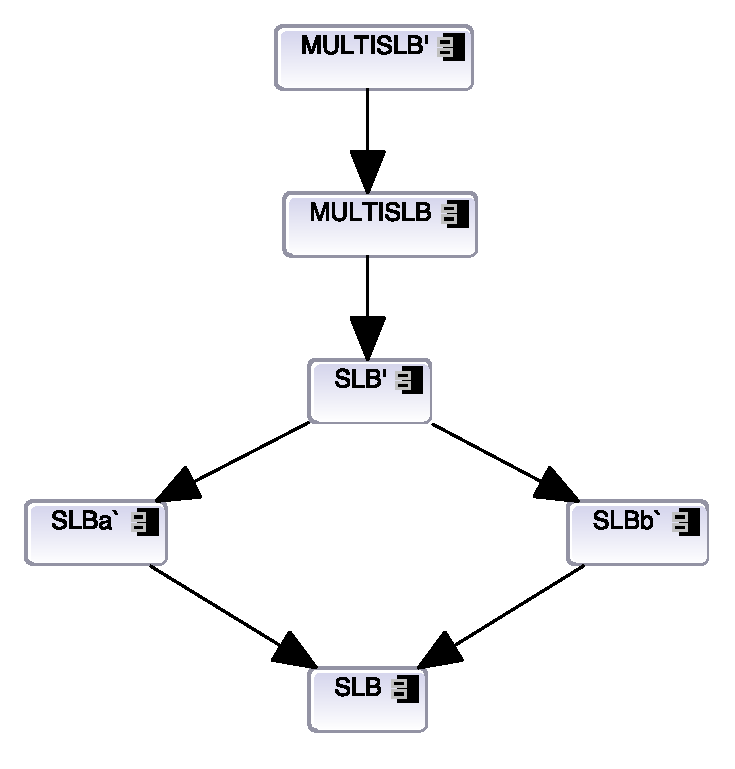
\includegraphics[width=0.6\columnwidth]{images/formal-corrected}
\par\end{centering}

\protect\caption{\label{fig:Correcting-any-compositional}Correcting any compositional
conflicts}


\end{figure}


The expanded graph is at the heart of our extension approach. In a
nutshell, replacement in an extension stratum allows us to insert
elements into an existing resemblance graph without directly editing
existing definitions. We can use replacement to effect changes to
compositional structure or to correct conflicts caused when we merge
branches.

The expanded graph specification relies on a notion of the topmost
definition of an element for a given perspective. In our original
example, from the \texttt{Single Lane Bridge} perspective, the topmost
definition of \texttt{SLB} is simply \texttt{SLB}. However, from the
perspective of \texttt{Merged} it is the set (\texttt{SLBa\textquoteright },
\texttt{SLBb\textquoteright }). To hold the topmost and expanded graph
information we add the following field to the \texttt{Stratum} structure:
\begin{lyxcode}
{\footnotesize{}sig~Stratum~\{}{\footnotesize \par}

{\footnotesize{}~~...}{\footnotesize \par}

{\footnotesize{}~~topmost:~Element~->~Element,}{\footnotesize \par}

{\footnotesize{}~~eresembles:~Element~->~Element,}{\footnotesize \par}

{\footnotesize{}~~...}{\footnotesize \par}

{\footnotesize{}\}}{\footnotesize \par}
\end{lyxcode}
\texttt{Topmost} is determined in the following way, where \texttt{s}
is the stratum perspective.
\begin{lyxcode}
{\footnotesize{}all~s:~Stratum,~e:~Element~\{}{\footnotesize \par}

{\footnotesize{}~~...}{\footnotesize \par}

{\footnotesize{}~~let~reps~=~replaces.e~\&~s.elements~|}{\footnotesize \par}

{\footnotesize{}~~~~some~reps~=>~s.topmost{[}e{]}~=~reps}{\footnotesize \par}

{\footnotesize{}~~~~~~else}{\footnotesize \par}

{\footnotesize{}~~~~e.home~=~s~=>~s.topmost{[}e{]}~=~e}{\footnotesize \par}

{\footnotesize{}~~~~~~else}{\footnotesize \par}

{\footnotesize{}~~~~s.topmost{[}e{]}~=~s.dependson.topmost{[}e{]}}{\footnotesize \par}

{\footnotesize{}~~...~}{\footnotesize \par}

{\footnotesize{}\}}{\footnotesize \par}
\end{lyxcode}
The first condition determines whether or not there is a replacement
of element \texttt{e} in \texttt{s}. If so, this is clearly the topmost
definition. Otherwise, if the perspective is the same as the element\textquoteright s
home stratum, then the topmost is simply the original element. Finally,
if none of these situations hold then we defer recursively to the
strata that the perspective depends upon\footnote{The \texttt{topmost} field and definition are effectively defining
a recursive function.}.

We can now compute \texttt{eresembles}, the expanded graph, using
the following logic.
\begin{lyxcode}
{\footnotesize{}let~joint~=~e.resembles~\&~ee.}{\footnotesize \par}

{\footnotesize{}~~~~replaces,rest~=~e.resembles~-~joint~|}{\footnotesize \par}

{\footnotesize{}~~s.eresembles{[}e{]}~=}{\footnotesize \par}

{\footnotesize{}~~~~e.home.dependson.topmost{[}joint{]}}{\footnotesize \par}

{\footnotesize{}~~~~+~s.topmost{[}rest{]}}{\footnotesize \par}
\end{lyxcode}
The \texttt{joint} set contains any elements that \texttt{e} is evolving
- i.e. where replacement and resemblance overlap. If we have evolution,
we need to look not at the current stratum (where \texttt{topmost}
would erroneously pick up the element \texttt{e} as a replacement),
but instead at the next lowest down strata in the dependency graph.
For all other resembled elements we can start at the current stratum.
It is also worth noting that for any replacement relation, the target
is the original unevolved element, even if another evolution of the
same element is visible to us underneath our home strata. This way,
even if we move the strata dependencies around we will not invalidate
any evolutions.


\subsection{Applying Deltas}

We are now in a position to apply the deltas by walking up the expanded
resemblance graph and adding, deleting and replacing constituents.
To hold the accumulated deltas we add the following fields to the
\texttt{Stratum} structure:
\begin{lyxcode}
{\footnotesize{}sig~Stratum~\{}{\footnotesize \par}

{\footnotesize{}~~...}{\footnotesize \par}

{\footnotesize{}~~edeltas:~Element~->~lone~Deltas,}{\footnotesize \par}

{\footnotesize{}~~full:~Element~->~Constituent~->~Constituent}{\footnotesize \par}

{\footnotesize{}\}}{\footnotesize \par}
\end{lyxcode}
For a given perspective \texttt{s}, element \texttt{e}, the deltas
from the expanded graph are accumulated into the \texttt{edeltas}
field as follows:
\begin{lyxcode}
{\footnotesize{}all~s:~Stratum,~e:~Element~\{}{\footnotesize \par}

{\footnotesize{}~~let~lower~=~s.eresembles{[}e{]},}{\footnotesize \par}

{\footnotesize{}~~~~~~me~=~s.edeltas{[}e{]}}{\footnotesize \par}

{\footnotesize{}~~\{}{\footnotesize \par}

{\footnotesize{}~~~~me.add~=~s.edeltas{[}lower{]}.add~+~e.deltas.add}{\footnotesize \par}

{\footnotesize{}~~~~me.delete~=~s.edeltas{[}lower{]}.delete}{\footnotesize \par}

{\footnotesize{}~~~~~~+~e.deltas.delete}{\footnotesize \par}

{\footnotesize{}~~~~me.replace~=~s.edeltas{[}lower{]}.replace}{\footnotesize \par}

{\footnotesize{}~~~~~~++~e.deltas.replace}{\footnotesize \par}

{\footnotesize{}~~~\}}{\footnotesize \par}

{\footnotesize{}\}}{\footnotesize \par}
\end{lyxcode}
In the above, we start with the element \texttt{e} from the perspective
\texttt{s}. We get the elements (\texttt{lower}) that \texttt{e} resembles
in the expanded graph. Then we form a new \texttt{Deltas} structure
(\texttt{edeltas}) by recursively summing up the deltas of the lower
elements and the deltas element of \texttt{e} itself - we union adds
and deletes and overwrite the lower replaces with the element\textquoteright s
replaces.

Finally, we form the complete structure (\texttt{full}) by finding
all topmost definitions of a given element \texttt{e}, and combining
the constituents by applying additions, replacements and finally deletions.
This order of application means that if one branch deletes a constituent
and another replaces it, then the deletion will always win out.
\begin{lyxcode}
{\footnotesize{}all~s:~Stratum,~e:~Element~\{}{\footnotesize \par}

{\footnotesize{}~~let~tops~=~s.topmost{[}e{]},~me~=~s.edeltas{[}tops{]}~|}{\footnotesize \par}

{\footnotesize{}~~~~some~e.replaces~=>~no~s.full{[}e{]}}{\footnotesize \par}

{\footnotesize{}~~~~~~else}{\footnotesize \par}

{\footnotesize{}~~~~s.full{[}e{]}~=}{\footnotesize \par}

{\footnotesize{}~~~~~~\{~a,~b:~me.add~|~a~=~b~\}}{\footnotesize \par}

{\footnotesize{}~~~~~~++~me.replace}{\footnotesize \par}

{\footnotesize{}~~~~~~-~\{~d:~me.delete,~allds:~Constituent~\}}{\footnotesize \par}

{\footnotesize{}\}}{\footnotesize \par}
\end{lyxcode}
The field \texttt{full} is actually a relation (\texttt{Constituent
- > Constituent}), reflecting that even if we replace a constituent
(right hand side) it still retains the identity of the original constituent
(left hand side). As described, this allows existing connectors to
stay valid. An addition of constituent \texttt{X} will result in an
\texttt{X -> X} entry.

The ability to express changes as deltas allows a component to completely
remake its inherited structure using a combination of adds, deletes
and replaces. Combined with the ability to remake an element\textquoteright s
resemblance graph using extension strata, an extension can adjust
the architecture of a system in any way it pleases without destructively
editing the original definition.


\subsection{Structural Conflicts}

Structural conflict occurs when two branches make incompatible evolutions
to the same element, and we then merge them into a common stratum.
For instance, \texttt{SLBa\textquoteright{}} might replace constituent
\texttt{X} with \texttt{Y} and \texttt{SLBb\textquoteright{}} might
replace \texttt{X} with \texttt{Z}. Upon merge, we retain both replacements,
and the full structure contains (\texttt{X -> Y}, and \texttt{X ->
Z}). When the \texttt{full} set of relations is not a partial function,
this type of conflict has occured- i.e. when we have more than one
range value for the same domain value in the set of relations.
\begin{lyxcode}
{\footnotesize{}pred~conflict{[}perspective:~Stratum,~e:~Element{]}~\{}{\footnotesize \par}

{\footnotesize{}~~not~functional{[}~perspective.full{[}e{]},~Element~{]}}{\footnotesize \par}

{\footnotesize{}\}}{\footnotesize \par}
\end{lyxcode}
This dilemma can be rectified by a subsequent evolution which definitively
replaces the constituent, say (\texttt{X -> Q}). This will overwrite
(\texttt{++}) all the previous entries that have \texttt{X} as the
domain value, as per the delta application rules.

More subtle conflicts occur when the adjusted structure in a branch
is compositionally incompatible with assumptions made in another branch.
For instance, one branch might delete a connector which the other
branch was relying on to be present. An expanded variant of the above
formal specification detects this by describing the actual component
model in terms of parts, ports, connectors and attributes rather than
generic constituents, and expressing well-formedness rules \cite{McVeigh2009}.


\subsubsection{Implementation of the Specification}

The Java runtime engine implementation of Backbone is based on the
expanded specification mentioned above, which additionally covers
areas such as the full component model, port type inference and interface
subtype rules. Of particular interest is the use of UUIDs to represent
element and constituent identity. Concretely, each constituent is
allocated a unique identifier, and when a constituent replaces this
it assumes the UUID of the replaced constituent. In the above specification
we have relied on direct element identity instead.


\subsubsection{Summary}

The formal specification explains how an extension stratum can affect
the resemblance graph of an existing element in an architecture. It
also details the rules via which delta application occurs, leading
to the full structure from a given stratum perspective. These rules
allow an extension stratum to control the way in which deltas of existing
elements are applied, allowing it to make any changes to the original
architecture required to support the extension.

\begin{comment}
\bibliographystyle{plain}
\bibliography{\string"/Users/amcveigh/Personal/evolve/Academic Work/read papers/references\string"}
\end{comment}

